\documentclass[onecolumn, letterpaper, 12pt]{article}
\usepackage{times,color,amsfonts,amsmath,amssymb,amsthm,comment,graphicx,cite,titlesec}
\usepackage{algorithm}
\usepackage{algpseudocode}
\usepackage{float}
\usepackage{fancyhdr} %%Fancy headings
\usepackage{setspace}

\singlespacing

\pagestyle{fancyplain}
\usepackage{listings} % Code output

\setlength{\parindent}{0.1in}
\setlength{\parskip}{0.05in}
\titleformat{\section}{\large\bfseries}{\thesection}{0.5em}{}
\titleformat{\subsection}{\bfseries}{\thesubsection}{0.5em}{}
\titleformat{\subsubsection}{\normalfont\bfseries}{\thesubsubsection}{0.5em}{}
\rhead{}
\lhead{}

\begin{document}

\thispagestyle{empty} %No headings/footers for the first pages.

\newcommand\reporttitle{Comparison of Multiple Sorting Algorithms}
\newcommand\reportauthor{Owen Miller-Fast}
\newcommand\due{13 November, 2022}


% Centered title page
\vfill
\begin{center}
	\hspace{0pt}
	\vfill
	\LARGE
	\reporttitle\\
	\reportauthor\\
	\due
	\normalfont
	\vfill
	\hspace{0pt}
	\pagebreak
\end{center}

\section{Motivation}
	\paragraph{}
	The amount of time an algorithm takes to produce a correct output can sometimes be the difference between life or death. For example, an air traffic controller collision detection process must be able to detect possible collisions as fast as possible, preferably real-time. The faster the algorithms can detect a possible collision, the less likely a collision will occur, saving countless lives.
	
	Knowing how fast an algorithm produces a correct result based on a large number of inputs is crucial when implementing large or time-critical programs.


\section{Background}
	\paragraph{}
	Many sorting algorithms exist, and they all do the same thing, sort a collection of data in a desired fashion, either that be ascending or descending. How does one choose which one to use? Usually, decisions are made with three concepts in mind, space complexity, time complexity, and ease of implementation.
	
	Insertion sort is an easy sort to implement but has bad time complexity, $O(n) = n^2$, and is slow with large inputs~\cite{cormen2001introduction}. In terms of time complexity, there are many better sorts than insertion sort; among these various sorts, this report will focus on merge, heap, and quicksort. Since the objective of this report is to analyze the time complexity of four separate sorts: merge, heap, quick, and a modified merge sort, space complexity will be ignored but is still important to keep in mind when implementing algorithms, especially those that are handling large amounts of data.
	
	It is guessed that quicksort will perform the fastest with random input, merge insertion sort with sorted input, and merge sort with reversely-sorted data.

\section{Procedure}
	\subsection{Psuedocode}
		\begin{algorithm}[H]
			\caption{\textsc{Swap}($n_1, n_2$)}
			\label{prot:swap}
			\begin{algorithmic}[1]
				\Procedure{Swap}{$n_1, n_2$}
					\State{$temp=n_1$}
					\State{$n_1=n_2$}
					\State{$n_2=temp$}
				\EndProcedure
			\end{algorithmic}
		\end{algorithm}
		\begin{algorithm}[H]
			\caption{\textsc{Insertion-Sort}($A, left, right$)}
			\label{prot:insertion-sort}
			\begin{algorithmic}[1]
				\Procedure{Insertion-Sort}{$A, left, right$}
					\State{assert($right-left\neq 0$)}
					\For{$j=left+1$ \textbf{to} $right-left$}
						\State{$key=A[j]$}
						\State{$i=j-1$}
						\While{$i>0$ \textbf{and} $A[i] > key$}
							\State{$A[i+1] = A[i]$}
							\State{$i=i-1$}
						\EndWhile
						\State{$A[i+1]=key$}
						\State{assert($A[left...j]$ is sorted)}
					\EndFor
					\State{assert($A[left...right]$ is sorted)}
				\EndProcedure
			\end{algorithmic}
		\end{algorithm}
		\begin{algorithm}[H]
			\caption{\textsc{Merge}($A, p, q, r$)}
			\label{prot:merge}
			\begin{algorithmic}[1]
				\Procedure{Merge}{$A, p, q, r$}
				\State{assert($A \neq \emptyset$)}
				\State{$n_1=q-p+1$}
				\State{$n_2=r-q$}
				\State{let $L[1...n_1+1]$ and $R[1...n_2+1]$ be new arrays}
				\For{$i=1$ \textbf{to} $n_1$}
				\State{$L[i]=A[p+i-1]$}
				\EndFor
				\For{$j=1$ \textbf{to} $n_2$}
				\State{$R[j]=A[q+j]$}
				\EndFor
				\State{$L[n_1+1]=\infty$}
				\State{$R[n_2+1]=\infty$}
				\State{$i=1$}
				\State{$j=1$}
				\For{$k=p$ \textbf{to} $r$}
				\If{$L[i]\le R[j]$}
				\State{$A[k]=L[i]$}
				\State{$i=i+1$}
				\Else
				\State{$A[k]=R[j]$}
				\State{$j=j+1$}
				\EndIf
				\State{// Current sub-array is sorted}
				\State{assert($\forall t : p < t \le k,  A[t-1] \le A[t])$}
				\State{// Every value in the sub-array is less than the values in \textit{L} and \textit{R}} 
				\State{assert($\forall t : p \le t \le k$ and $\forall a : i \le a \le n_1, A[t] \le L[a]$)}
				\State{assert($\forall t : p \le t \le k$ and $\forall b : j \le b \le n_2, A[t] \le R[b]$)}
				\EndFor
				\State{// $A[p...r]$ is sorted}
				\State{assert($\forall t : p < t \le r,  A[t-1] \le A[t]$)}
				\EndProcedure
			\end{algorithmic}
		\end{algorithm}
		\begin{algorithm}[H]
			\caption{\textsc{Max-Heapify}($A, i$)}
			\label{prot:heapify}
			\begin{algorithmic}[1]
				\Procedure{Heapify}{$A, i$}
				\State{assert($A \neq \emptyset$)}
				\State{$l=\textsc{LEFT}(i)$}
				\State{$r=\textsc{RIGHT}(i)$}
				\If{$l \le$ \textit{A.heap-size} \textbf{and} $A[l] > A[i]$}
				\State{$largest=l$}
				\Else
				\State{$largest=i$}
				\EndIf
				\If{$r \le$ \textit{A.heap-size} \textbf{and} $A[r] > A[largest]$}
				\State{$largest=r$}
				\EndIf
				\If{$largest\neq i$}
				\State{$\textsc{SWAP}(A[i], A[largest])$}
				\State{$\textsc{MAX-HEAPIFY}($\textit{A.largest}$)$}
				\EndIf
				\State{assert($i$ is a root of a max heap)}
				\EndProcedure
			\end{algorithmic}
		\end{algorithm}
		\begin{algorithm}[H]
			\caption{\textsc{Build-Max-Heap}($A$)}
			\label{prot:build-heap}
			\begin{algorithmic}[1]
				\Procedure{Build-Heap}{$A$}
				\State{assert($A \neq \emptyset$)}
				\State{\textit{A.heap-size} $ = A.length$}
				\State{// Root is trivially a max heap}
				\For{$i=\lfloor A.length/2\rfloor$ \textbf{downto} $1$}
				\State{$\textsc{MAX-HEAPIFY}(A, i)$}
				\State{assert($i$ is the root of a max heap)}
				\EndFor
				\State{assert($\forall t : 1 \le t \le A.length, A[t]$ is the root of a max heap)}
				\EndProcedure
			\end{algorithmic}
		\end{algorithm}
		\begin{algorithm}[H]
			\caption{\textsc{Partition}($A, p, r$)}
			\label{prot:part}
			\begin{algorithmic}[1]
				\Procedure{Partition}{$A, p, r$}
				\State{assert($A \neq \emptyset$)}
				\State{$x=A[r]$}
				\State{$i=p-1$}
				\For{$j=p$ \textbf{to} $r-1$}
				\If{$A[j]\le x$}
				\State{$i=i+1$}
				\State{$\textsc{SWAP}(A[i], A[j])$}
				\State{assert($\forall t : p \le t \le j, A[t] \le x$)}
				\EndIf
				\State{assert($\forall t : i < t < j, A[t] > x$)}
				\EndFor
				\State{// Since $j=r$, every value is partitioned into correct sets}
				\State{$\textsc{SWAP}(A[i+1], A[r])$}
				\State{\textbf{return} $i+1$}
				\EndProcedure
			\end{algorithmic}
		\end{algorithm}
		\begin{algorithm}[H]
			\caption{\textsc{Merge-Sort}($A, p, r$)}
			\label{prot:merge-sort}
			\begin{algorithmic}[1]
				\Procedure{Merge-Sort}{$A, p, r$}
					\State{assert($A \neq \emptyset$)}
					\If{$p < r$}
						\State{$q = \lfloor (p+r)/2 \rfloor$}
						\State{\textsc{MERGE-SORT}($A, p, q$)}
						\State{\textsc{MERGE-SORT}($A, q + 1, r$)}
						\State{\textsc{MERGE}($A, p, q, r$)}
					\EndIf
				\EndProcedure
			\end{algorithmic}
		\end{algorithm}
		\begin{algorithm}[H]
			\caption{\textsc{Heap-Sort}($A$)}
			\label{prot:heap-sort}
			\begin{algorithmic}[1]
				\Procedure{Heap-Sort}{$A$}
					\State{assert($A \neq \emptyset$)}
					\State{$\textsc{BUILD-MAX-HEAP}(A)$}
					\For{$i=A.length$ \textbf{downto} $2$}
						\State{$\textsc{SWAP}(A[1], A[i])$}
						\State{\textit{A.heap-size} $=$ \textit{A.heap-size} $-1$}
						\State{$\textsc{MAX-HEAPIFY}(A, 1)$}
					\EndFor
					\State{assert($\forall t : 1 < t \le A.length,  A[t-1] \le A[t]$)}
				\EndProcedure
			\end{algorithmic}
		\end{algorithm}
		\begin{algorithm}[H]
			\caption{\textsc{Quick-Sort}($A, p, r$)}
			\label{prot:quick-sort}
			\begin{algorithmic}[1]
				\Procedure{Quick-Sort}{$A, p, r$}
					\State{assert($A \neq \emptyset$)}
					\If{$p < r$}
						\State{$q=\textsc{PARTITION}(A, p, r)$}
						\State{$\textsc{QUICK-SORT}(A, p, q-1)$}
						\State{$\textsc{QUICK-SORT}(A, q+1, r)$}
					\EndIf
					\State{assert($\forall t : 1 < t \le r,  A[t-1] \le A[t]$)}
				\EndProcedure
			\end{algorithmic}
		\end{algorithm}
		\begin{algorithm}[H]
			\caption{\textsc{Merge-Insertion-Sort}($A, left, right$)}
			\label{prot:merge-insertion-sort}
			\begin{algorithmic}[1]
				\Procedure{Merge-Insertion-Sort}{$A, left, right$}
					\State{$A\neq \emptyset$}
					\If{$(right-left)>43$}
						\State{$middle=\lfloor (p+r)/2\rfloor$}
						\State{$\textsc{MERGE-SORT}(A, p, q)$}
						\State{$\textsc{MERGE-SORT}(A, p, q)$}
						\State{$\textsc{MERGE}(A, p, q, r)$}
					\Else
						\State{$\textsc{INSERTION-SORT}(A, left, right)$}
					\EndIf
				\EndProcedure
			\end{algorithmic}
		\end{algorithm}
	\subsection{Preconditions, Postconditions, and Invariants}
		\subsubsection{\textsc{Insertion-Sort}$(A, left, right)$}
			\footnotesize
			Algorithm~\ref{prot:insertion-sort}\\
			\textbf{Precondition}: Sub-array is not empty\\
			\textbf{Postcondition}:$A[left...right]$ is sorted in ascending order\\
			\textbf{Invariant}: $A[left...j-1]$ is in ascending order
			\begin{itemize}
				\item \textbf{Initialization}: Plug $j=left+1$ in $A[left...j-1]$, $A[left...left]$ is trivially sorted
				\item \textbf{Maintenance}: At the beginning of each iteration, $A[left...j-1]$ is sorted. The algorithm works by moving the values $A[j-1], A[j-2], A[j-n]$ to the right until it finds the proper place for $A[j]$, at which it inserts $A[j]$ into sorted array, making $A[left...j]$ sorted.
				\item \textbf{Termination}: At termination, $j=(right-left)+1$. Plug $j$ into the invariant, $A[left...(right-left)+1-1]$ or $A[left...(right-left)]$ is sorted.
			\end{itemize}
			\normalsize
		\subsubsection{\textsc{Merge}$(A, p, q, r)$}
			\footnotesize
			Algorithm~\ref{prot:merge}\\
			\textbf{Precondition}: $A$ is not empty\\
			\textbf{Postcondition}:$A[p...r]$ is sorted in ascending order\\
			\textbf{Invariant}: The start of each iteration of the \textbf{for} loop of lines 16-22, the sub-array $A[p...k-1]$ contains the $k-p$ smallest elements of $L$ and $R$ in sorted order. Additionally, $L[i]$ and $R[j]$ are the smallest values in their respective arrays that have not been copied back yet.
			\begin{itemize}
				\item \textbf{Initialization}: $A[p...k-1]$ is empty and since $i=j=1$, no elements from $L$ or $R$ have been copied back to $A$
				\item \textbf{Maintenance}: Each iteration of the loop copies the smallest value from $L$ or $R$ into $A[k]$. After the smallest value, $R[j]$ or $L[i]$, is copied to $A[k]$, $k$ and the respective array accessor, $j$ or $i$, is incremented, making the sub-array $A[p...k]$ sorted and upholding the invariant.
				\item \textbf{Termination}: At termination, $k=r+1$. If plugged into the loop invariant, $A[p...(r+1)-1]$ or $A[p...r]$ is sorted. $A[p...r]$ contains the $k-p=r-p+1$ smallest elements of $L$ and $R$ in sorted order
			\end{itemize}
			\normalsize
		\subsubsection{\textsc{Max-Heapify}$(A, i)$}
			\footnotesize
			Algorithm~\ref{prot:heapify}\\
			\textbf{Precondition}: $A$ is not empty and $2i$ and $2i+1$ are roots of a max heap\\
			\textbf{Postcondition}: $i$ is a root of a max heap and its children are smaller than it
			\normalsize
		\subsubsection{\textsc{Build-Max-Heap}$(A)$}
			\footnotesize
			Algorithm~\ref{prot:build-heap}\\
			\textbf{Precondition}: $A$ is not empty\\
			\textbf{Postcondition}: $A[1]$ is the root of a max heap\\
			\textbf{Invariant}: At the start of each iteration of the \textbf{for} loop of lines 5-7, each node is the root of a max heap.
			\begin{itemize}
				\item \textbf{Initialization}: Each node $\lfloor n/2\rfloor + 1,\lfloor n/2\rfloor + 2,\lfloor n/2\rfloor + 3...n$ is a leaf and trivially a max heap.
				\item \textbf{Maintenance}: $i$'s children are numbered higher than it, they are roots of max heaps. \textsc{MAX-HEAPIFY} preserves this. Decrementing $i$ reestablishes the loop invariant. 
				\item \textbf{Termination}: At termination, $i=0$. Plugged into the invariant, $1,2,3,...n$ are roots of a max heap. Primarily, $A[1]$
			\end{itemize}
			\normalsize
		\subsubsection{\textsc{Partition}$(A, p, r)$}
			\footnotesize
			Algorithm~\ref{prot:part}\\
			\textbf{Precondition}: $A$ is not empty\\
			\textbf{Postcondition}: $A[p...r]$ partitioned into three sections\textbackslash sets\\
			\textbf{Invariant}: At the beginning of each iteration of the loop of lines 5-9, for any array index $k$:
			\begin{enumerate}
				\item If $p \le k\le i,$ then $A[k] \le x$
				\item If $i+1\le k\le j-1,$ then $A[k] > x$
				\item If $k=r,$ then $A[k]=x$
			\end{enumerate}
			\begin{itemize}
				\item \textbf{Initialization}: $i = p-1$ and $j=p$. No values lie in between $i$ and $j$ so the conditions for the invariant is trivially satisfied.
				\item \textbf{Maintenance}: If $A[j]\le x$, $A[i] is swapped with A[j]$ and $i$ is incremented, satisfying condition 1 and 2 of the loop invariant
				\item \textbf{Termination}: At termination, $j=r$. Therefore, every entry in the array is in one of the three sets described by the loop invariant.
			\end{itemize}
			\normalsize
		\subsubsection{\textsc{Merge-Sort}$(A, p, r)$}
			\footnotesize
			Algorithm~\ref{prot:merge-sort}\\
			\textbf{Precondition}: $A$ is not empty\\
			\textbf{Postcondition}: $A$ is sorted in ascending order
			\normalsize
		\subsubsection{\textsc{Heap-Sort}$(A)$}
			\footnotesize
			Algorithm~\ref{prot:heap-sort}\\
			\textbf{Precondition}: $A$ is not empty\\
			\textbf{Postcondition}: $A$ is sorted in ascending order
			\normalsize
		\subsubsection{\textsc{Quick-Sort}$(A, p, r)$}
			\footnotesize
			Algorithm~\ref{prot:quick-sort}\\
			\textbf{Precondition}: $A$ is not empty\\
			\textbf{Postcondition}: $A$ is sorted in ascending order
			\normalsize
		\subsubsection{\textsc{Insertion-Merge-Sort}$(A, left, right)$}
			\footnotesize
			Algorithm~\ref{prot:merge-insertion-sort}\\
			\textbf{Precondition}: $A$ is not empty\\
			\textbf{Postcondition}: $A$ is sorted in ascending order
	\normalsize
	\subsection{General Idea}
		\paragraph{}
		To time how long an algorithm takes on a machine, one would ideally isolate algorithm to avoid interference from different running processes. It is next to impossible on current operating systems since the OS is usually executing other processes concurrent to the algorithm. 
		
		To combat this, the average of runs on input size $n$ can be computed, more detail on this in \textit{Section 5.1}. Each algorithms' invariants, preconditions, and postconditions were included in the code either as an if or assert statement. To test if an array or a sub-array is sorted, the \textit{algorithms} library was used (\textit{is\_sorted()}).
\section{Testing}
	\subsection{Testing Plan and Results}
		Each sorting algorithm except quicksort:\\\\
		\small{\begin{tabular}{|l|l|l|l|}
		\hline Test input & Expected Results & Actual Results & Corrective Actions \\ 
		\hline  Empty array & Nothing returned  & Nothing was returned & No action taken  \\ 
		\hline All elements identical & Same array  & Same array returned & No action taken  \\ 
		\hline Max array size & Sorted array & Sorted array returned & No action taken \\
		\hline
		\end{tabular}}\\
		
		\noindent quicksort:\\\\
		\small{\begin{tabular}{|l|l|l|l|}
		\hline Test input & Expected Results & Actual Results & Corrective Actions \\
		\hline Empty array & Nothing returned & Nothing was returned & No action taken \\
		\hline Array size of 20,000 & Sorted array & Sorted array returned & No action taken \\
		\hline Array size of 35,000 & Sorted array & Segmentation fault & Increase max stack size \\
		\hline Max array size & Sorted array & Segmentation fault & Increase max stack size \\
		\hline
		\end{tabular}}
	\normalsize
	\subsection{Problems Encountered}
		\paragraph{}
		Contrary to the first project, many problems were encountered. There were two main problems: algorithms appearing linear and quicksort randomly segmentation faults. A solution was found for quicksort randomly faulting. The algorithms appearing linear was a problem until analysis on them were done and they were actually not linear.
		
		Next, the quicksort randomly segmentation faulting was caused by Windows' max stack limit, 1MB. Once a program hits the maximum stack limit, it is killed. Quicksort, especially when the array is sorted or reversely-sorted, creates many function calls on the call stack. Once the maximum was reached, the program would segmentation fault. To combat that, the program must be compiled with an increase of max stack size.

\section{Experimental Analysis}
	\normalsize
	\subsection{Process Description}
		\paragraph{}
		The documented code used to generate the data presented in this report is in Appendix A and will be referenced multiple times throughout Section 5. The merge, heap, quick, and modified merge sort is located in mergeSort(), heapSort(), quickSort(), and mergeInsertionSort() functions respectfully. 
		
		To enforce preconditions, postconditions, and invariants, \textit{if} and \textit{assert} statements were included in the algorithms' main and auxiliary functions. If \textit{am.debug} is set to true, the program will run each \textit{assert} and \textit{if} statement to ensure the correctness of the algorithms. It can be toggled since checking algorithms' correctness can skew results.
		
		To determine the theoretical speed for merge, heap, quick, and modified merge sort, their respective recurrence functions must be solved. Simply enough, every algorithms' recurrence function is $T(n)=aT(\dfrac{n}{b}) + O(n)$, $a=b$. Solving this recurrence function using the Master's Theorem gives the solution: $T(n)=O(cnlgn)$. It is important to note, however, that quicksort's worst case is $O(n^2)$ when the array is sorted and reversely-sorted since the recurrence function for quicksort's worst case is $T(n)=2T(\dfrac{n}{2}) + O(cn^2)$, which is $O(n^2)$. Since every algorithms' time is $O(cnlgn)$, one can only be faster if their constant is smaller than the others' constant; this is what this report hopes to examine and determine.
		
		The \textit{chrono} library was used to time the algorithms. Before calling the algorithm through a dynamic pointer, the variable \textit{start} is created to record the time before execution. After execution, the variable \textit{end} is created to record the time after execution. The variable \textit{duration} stored the difference between \textit{end} and \textit{start}, which represented how long it took for the algorithms to complete.
		
		Since running the algorithm in isolation is virtually impossible, averaging the time the algorithm takes at each input size, $n$, can mitigate the interference from other running processes. \textit{AlgorithmManager} has internal variables \textit{average}, \textit{randomResults}, \textit{sortedResults}, and \textit{reverseReults} that handle averaging and storing time values of each algorithm at each input size, $n$.
		
		The program \textbf{must} be ran with five inputs: name of the file with the to-be-sorted data in it, starting size, max size, size of increments, and how many times the algorithm will run at each input $n$. Note, the type of data in the file must match the data type of \textit{AlgorithmManager} and the data structure holding the data at compile time.
		
		Within the main cpp file, \textit{am.timeAlgorithm()} is called with arguments of type \textit{Algorithm} and \textit{int}. \textit{Algorithm} is an enumerator that describes which algorithm is being tested. Using a switch statement, \textit{timeAlgorithm()} dynamically points to a wrapper that calls the specified function; this cut down on the number of lines in the program. The \textit{int} argument is the number of times the algorithm will be tested at input size, $n$.
		
		Each algorithm is tested against an random, sorted, and reversely-sorted array. The time values of each are exported after all the testing is done using the \textit{am.exportResults()} function. The \textit{exportResults()} function takes a \textit{string} argument that simply names the .csv outputted.
		
		Due to time constraints, every algorithm was ran 15 times per input size, $n$, with an initial size, $n_0$, of 150 to a maximum size of 30,000, incremented by 150. The algorithms' constant is labeled on each figure and will compared to find the fastest algorithm.
	\subsection{Merge Sort}
		\paragraph{}
		The merge sort algorithm works by dividing an array in halves until the sub-arrays are of length one. Once the sub-arrays are of length one, \textsc{MERGE} merges the sub-arrays together where the values in each sub-array are in sorted order.
		\subsubsection{Random Case}
			\paragraph{}
			The results of merge sort sorting a random array is shown in Figure~\ref{graph:merge-random}. Merge sort on a random array is $O(cnlgn)$. As seen in Figure~\ref{graph:merge-random}, the constant value, $c$, is 18.5962. This value was found solving the equation $y=cnlgn$ where $y$ is the max time value and $n$ is max input value. In this case, $y=8297260$ and $n=30000$. 
			\begin{figure}[H]
				\centering
				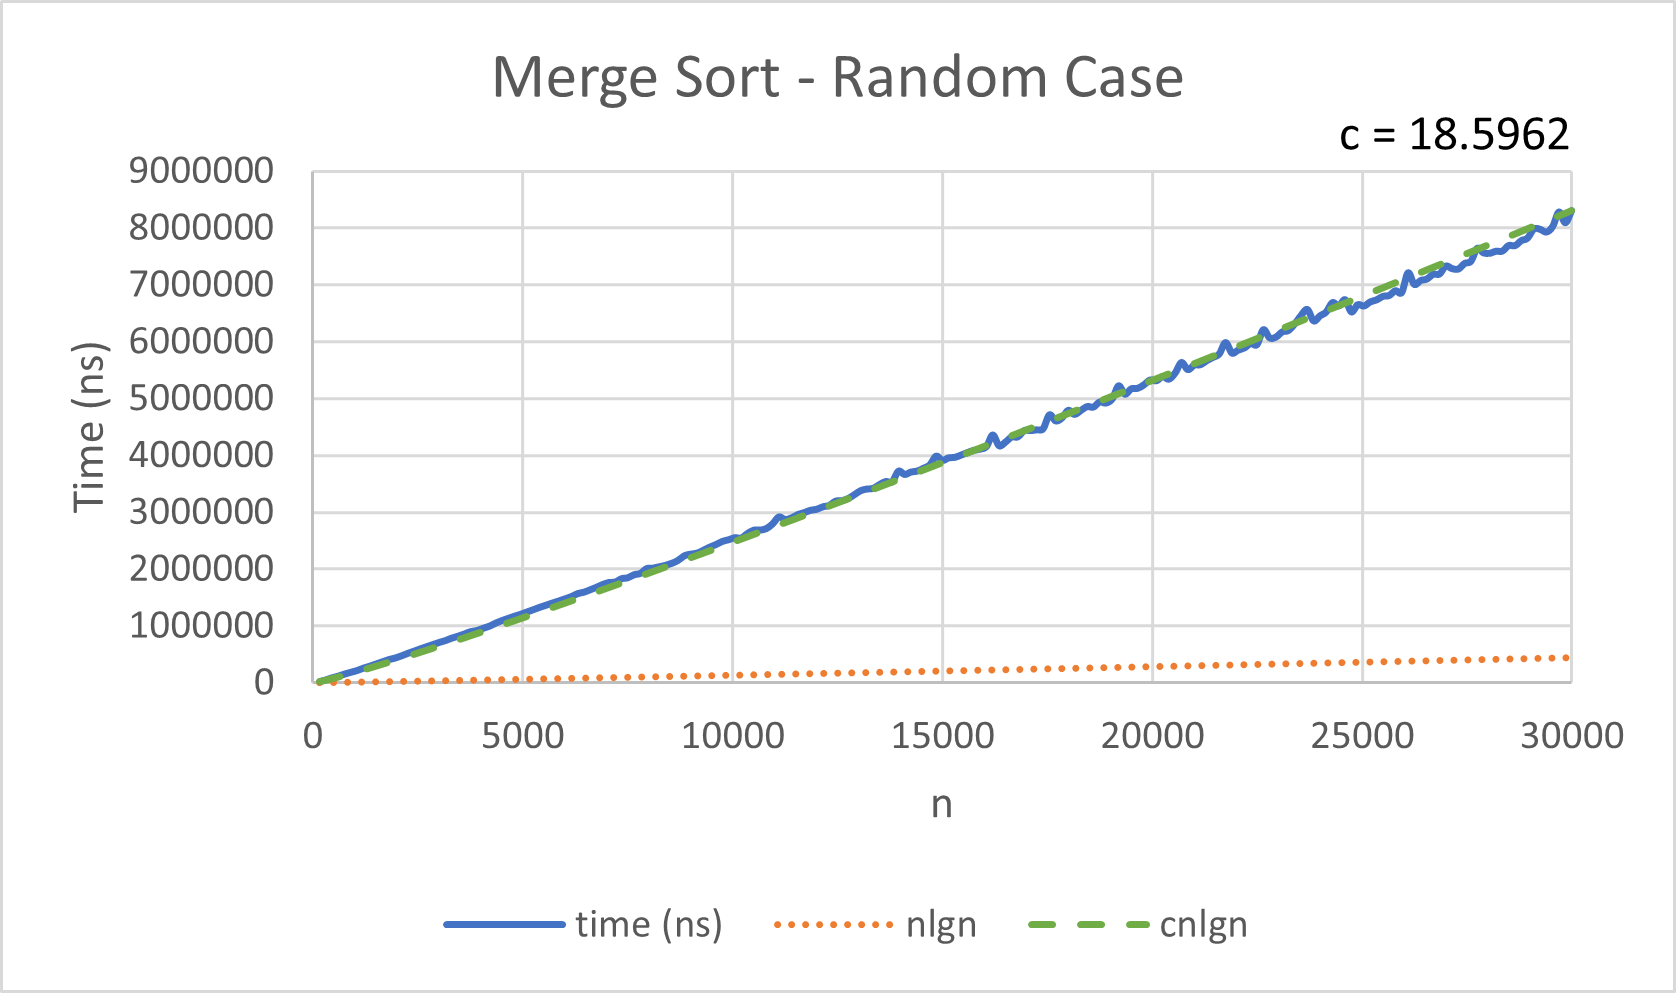
\includegraphics[width=0.9\linewidth]{merge_random.png}
				\caption{Merge Sort - Random Case}
				\label{graph:merge-random}
			\end{figure}
		\subsubsection{Sorted Case}
			\paragraph{}
			The results of merge sort sorting a sorted array is shown in Figure~\ref{graph:merge-sorted}. Merge sort on a sorted array is $O(cnlgn)$. As seen in Figure~\ref{graph:merge-sorted}, the constant value, $c$, is 14.18871. This value was found solving the equation $y=cnlgn$ where $y=$ the max time value and $n=$ max input value. In this case, $y=6213450$ and $n=30000$. 
			\begin{figure}[H]
				\centering
				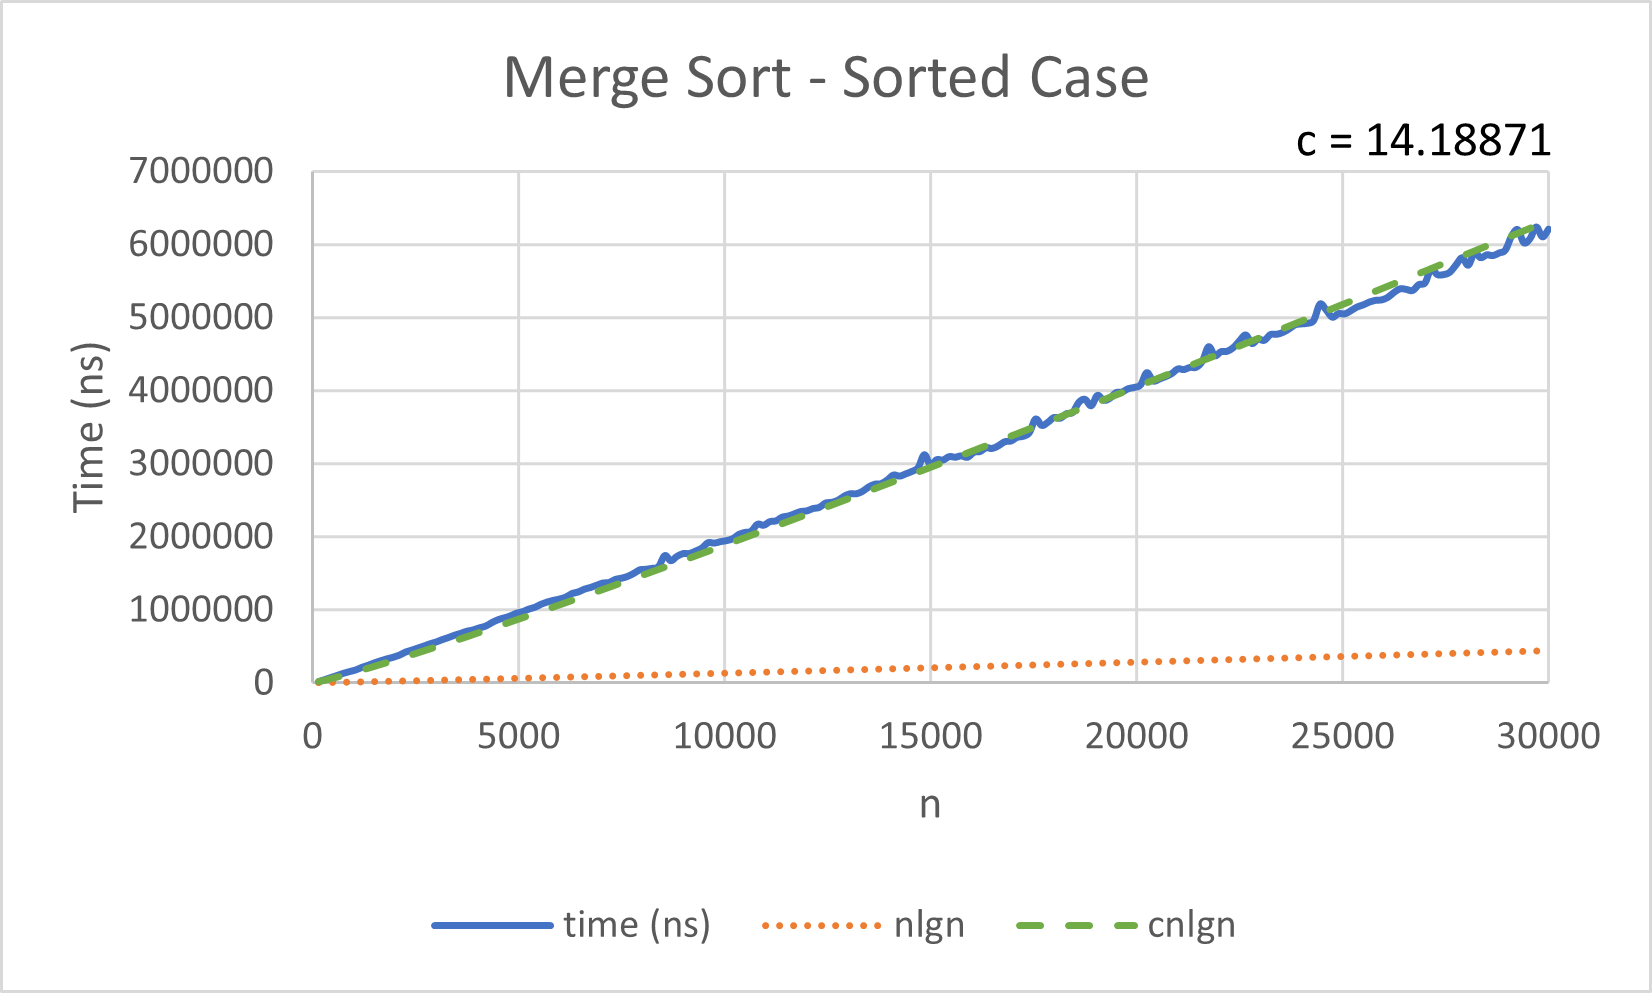
\includegraphics[width=0.9\linewidth]{merge_sorted.png}
				\caption{Merge Sort - Sorted Case}
				\label{graph:merge-sorted}
			\end{figure}
		\subsubsection{Reverse Case}
			\paragraph{}
			The results of merge sort sorting a reversely-sorted array is shown in Figure~\ref{graph:merge-reverse}. Merge sort on a reversely-sorted array is $O(cnlgn)$. As seen in Figure~\ref{graph:merge-reverse}, the constant value, $c$, is 14.102. This value was found solving the equation $y=cnlgn$ where $y$ is the max time value and $n$ is max input value. In this case, $y=6292040$ and $n=30000$. 
			\begin{figure}[H]
				\centering
				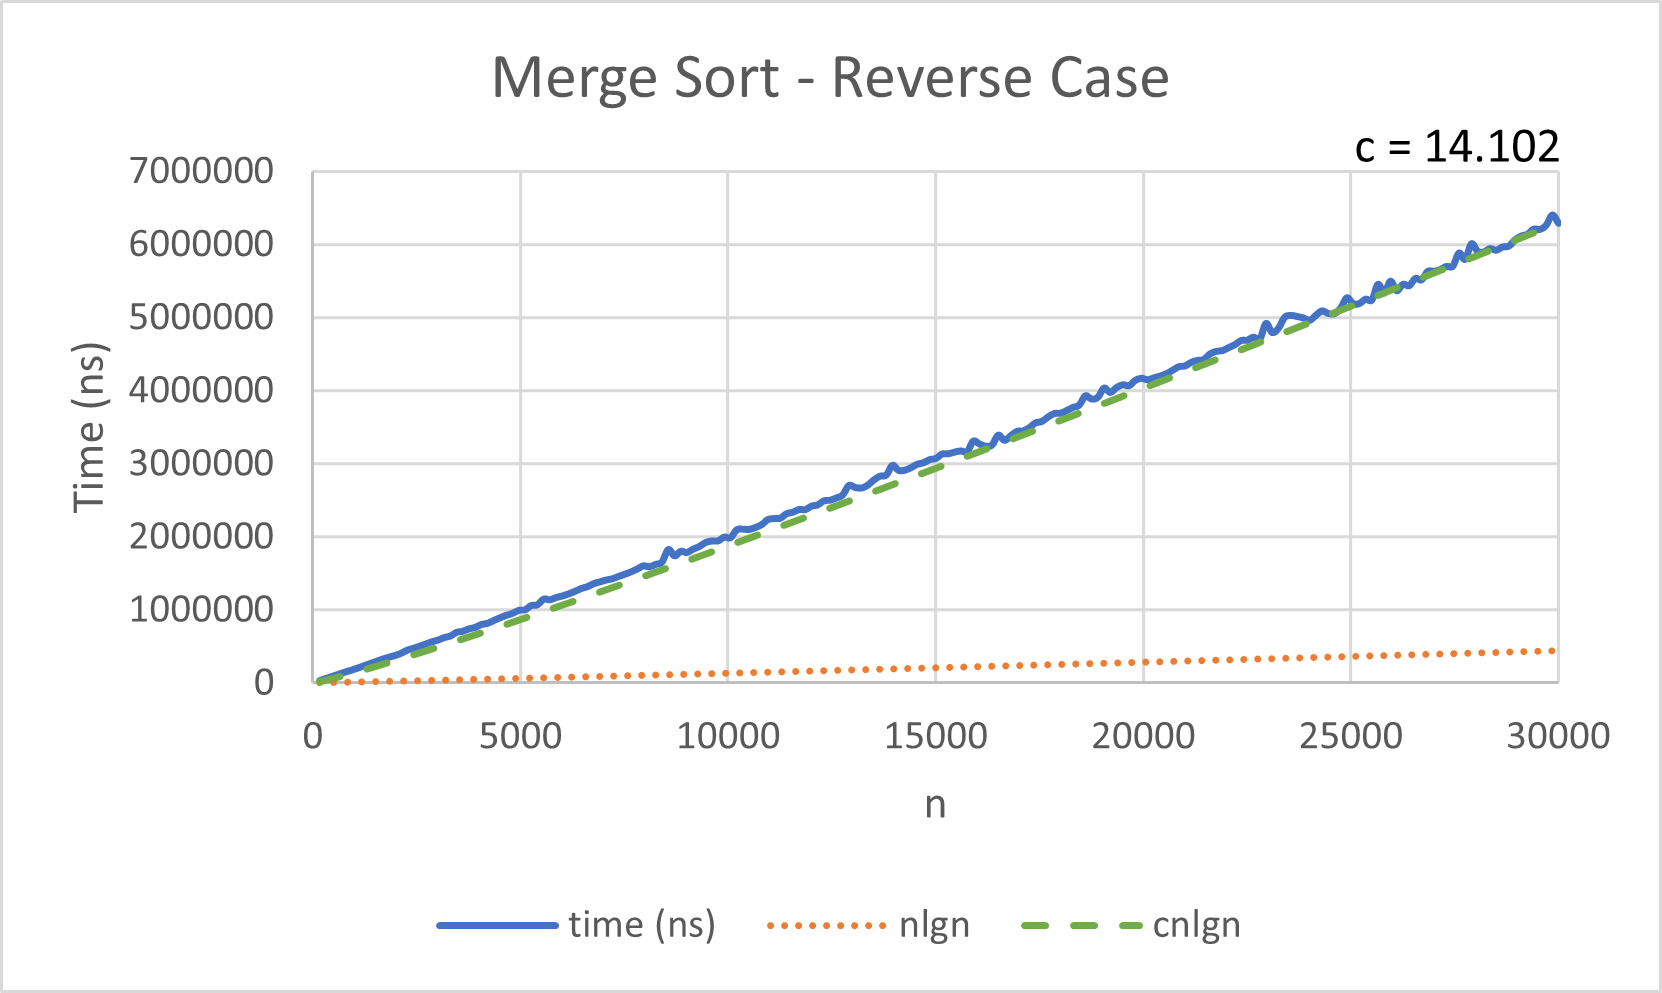
\includegraphics[width=0.9\linewidth]{merge_reverse.png}
				\caption{Merge Sort - Reverse Case}
				\label{graph:merge-reverse}
			\end{figure}
	\subsection{Heap Sort}
		\paragraph{}
		The heap sort algorithm works by exploiting the nature of how a maximum heap is stored in an array. The algorithm will \textsc{HEAPIFY} an array, move the first element to the back of the array, and repeat the process for the remaining sub-array.
		\subsubsection{Random Case}
			\paragraph{}
			The results of heap sort sorting a random array is shown in Figure~\ref{graph:heap-random}. Heap sort on a random array is $O(cnlgn)$. As seen in Figure~\ref{graph:heap-random}, the constant value, $c$, is 16.12624. This value was found solving the equation $y=cnlgn$ where $y$ is the max time value and $n$ is max input value. In this case, $y=7195210$ and $n=30000$. 
			\begin{figure}[H]
				\centering
				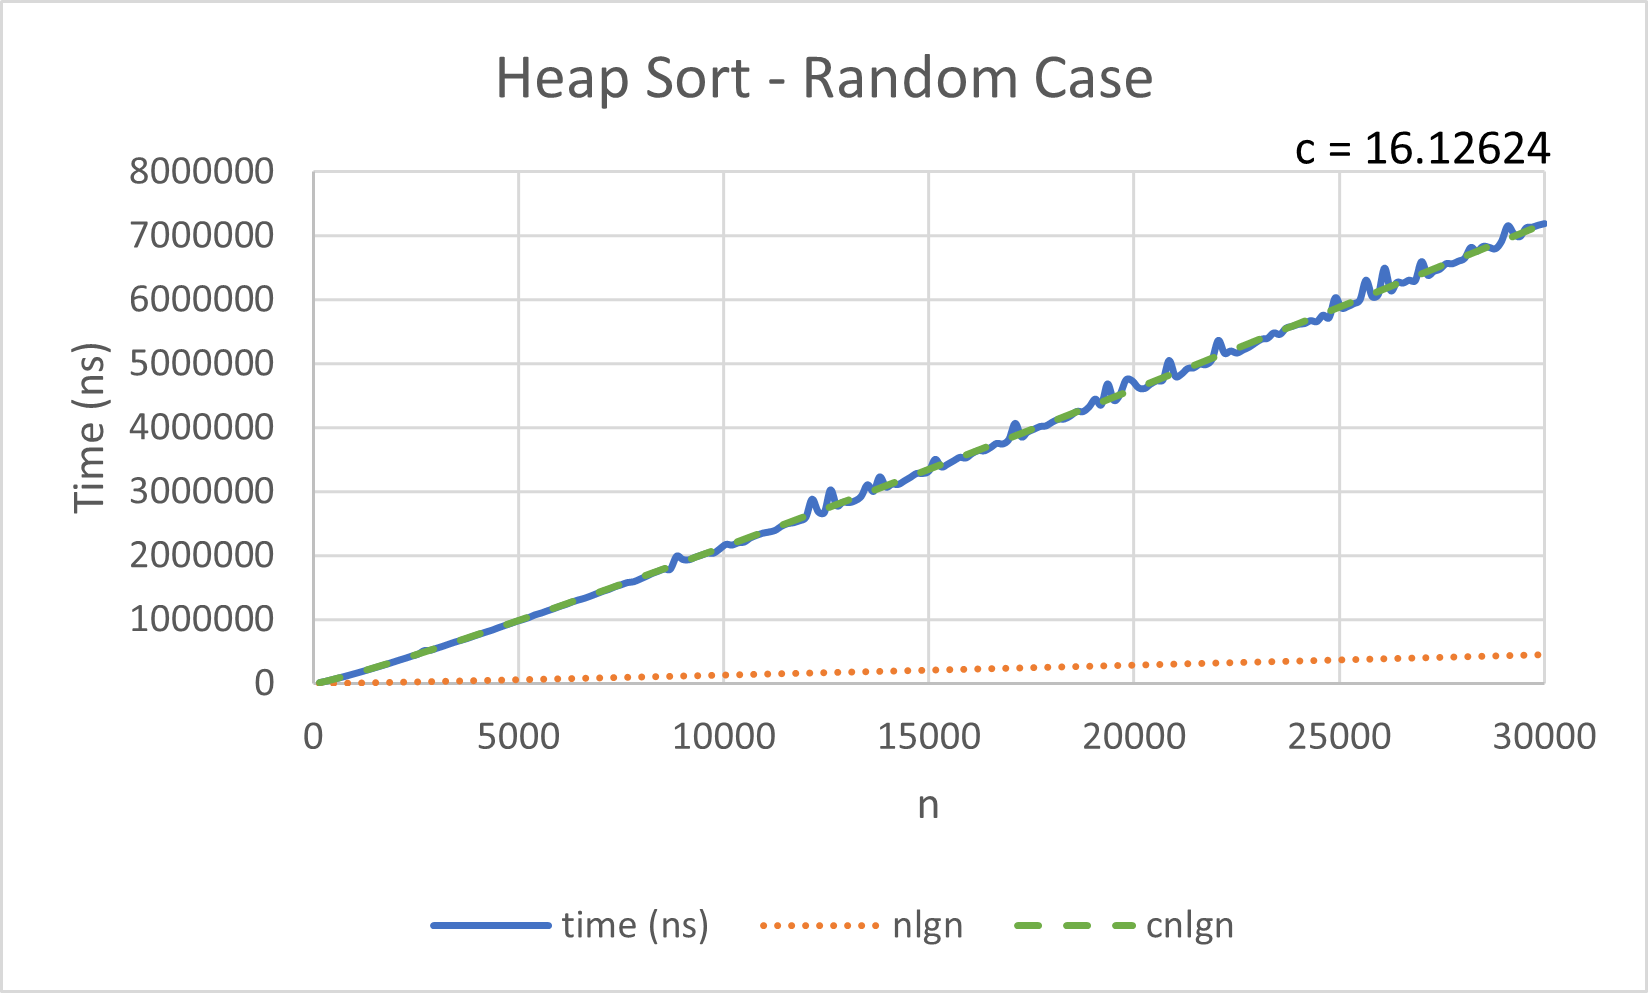
\includegraphics[width=0.9\linewidth]{heap_random.png}
				\caption{Heap Sort - Random Case}
				\label{graph:heap-random}
			\end{figure}
		\subsubsection{Sorted Case}
			\paragraph{}
			The results of heap sort sorting a sorted array is shown in Figure~\ref{graph:heap-sorted}. Heap sort on a sorted array is $O(cnlgn)$. As seen in Figure~\ref{graph:heap-sorted}, the constant value, $c$, is 14.18871. This value was found solving the equation $y=cnlgn$ where $y$ is the max time value and $n$ is max input value. In this case, $y=6330720$ and $n=30000$. 
			\begin{figure}[H]
				\centering
				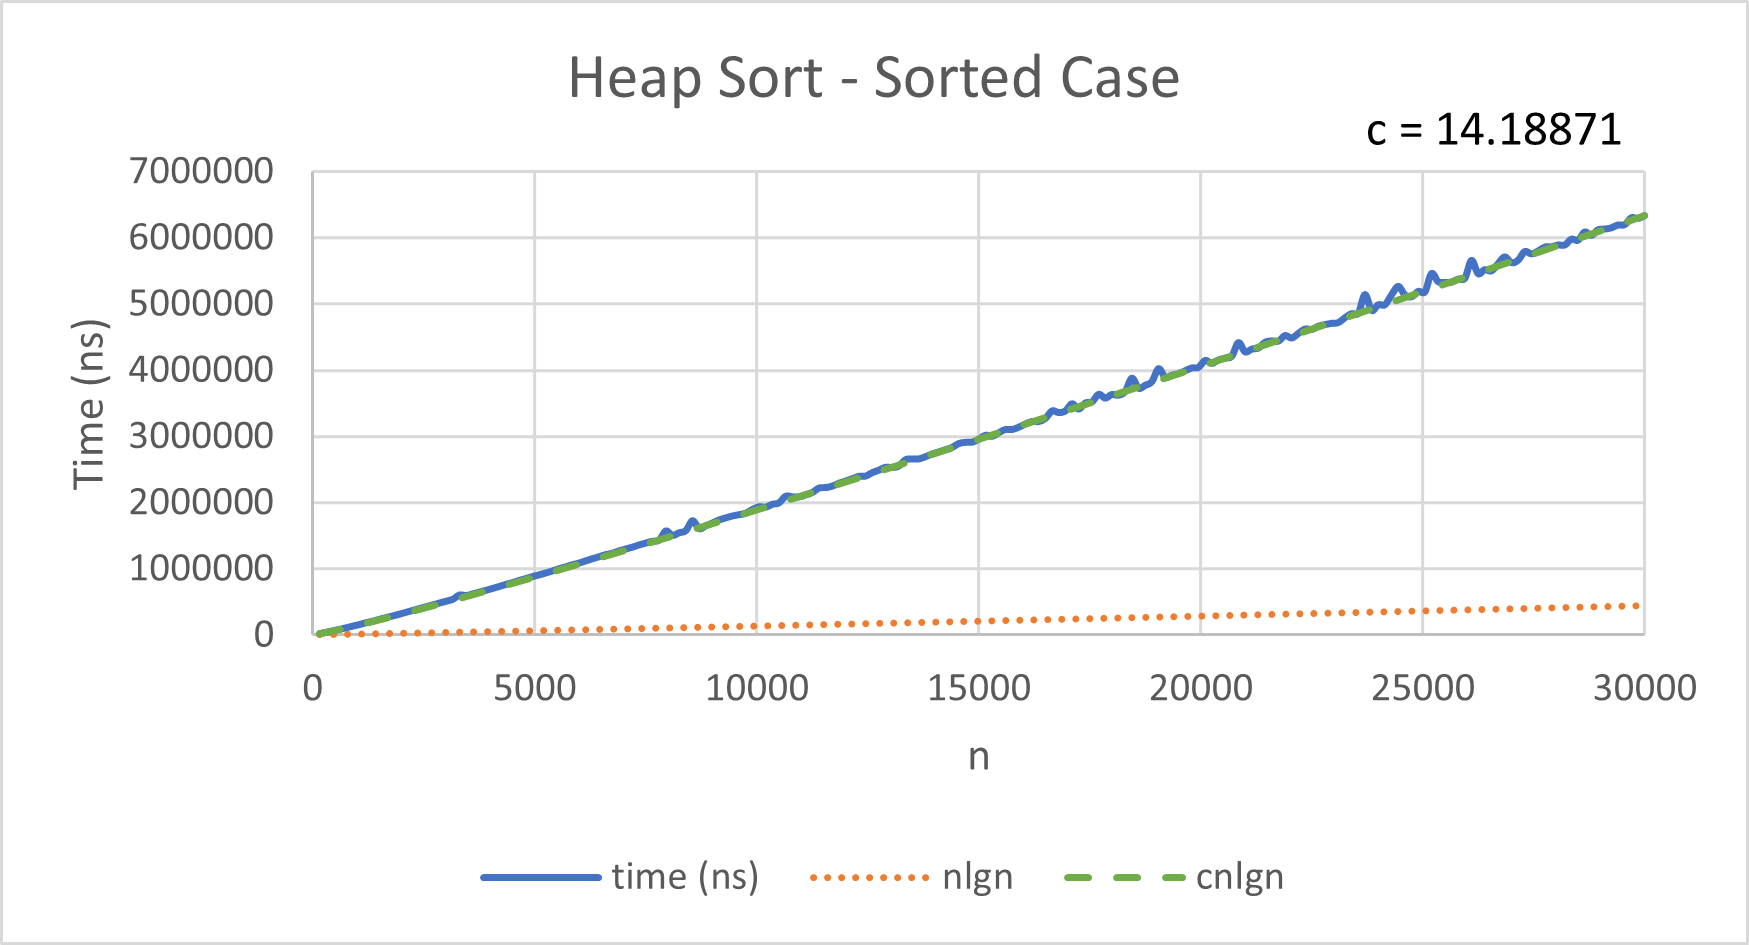
\includegraphics[width=0.9\linewidth]{heap_sorted.png}
				\caption{Heap Sort - Sorted Case}
				\label{graph:heap-sorted}
			\end{figure}
		\subsubsection{Reverse Case}
			\paragraph{}
			The results of heap sort sorting a reversely-sorted array is shown in Figure~\ref{graph:heap-reverse}. Heap sort on a reversely-sorted array is $O(cnlgn)$. As seen in Figure~\ref{graph:heap-reverse}, the constant value, $c$, is 13.39651. This value was found solving the equation $y=cnlgn$ where $y$ is the max time value and $n$ is max input value. In this case, $y=5977260$ and $n=30000$. 
			\begin{figure}[H]
				\centering
				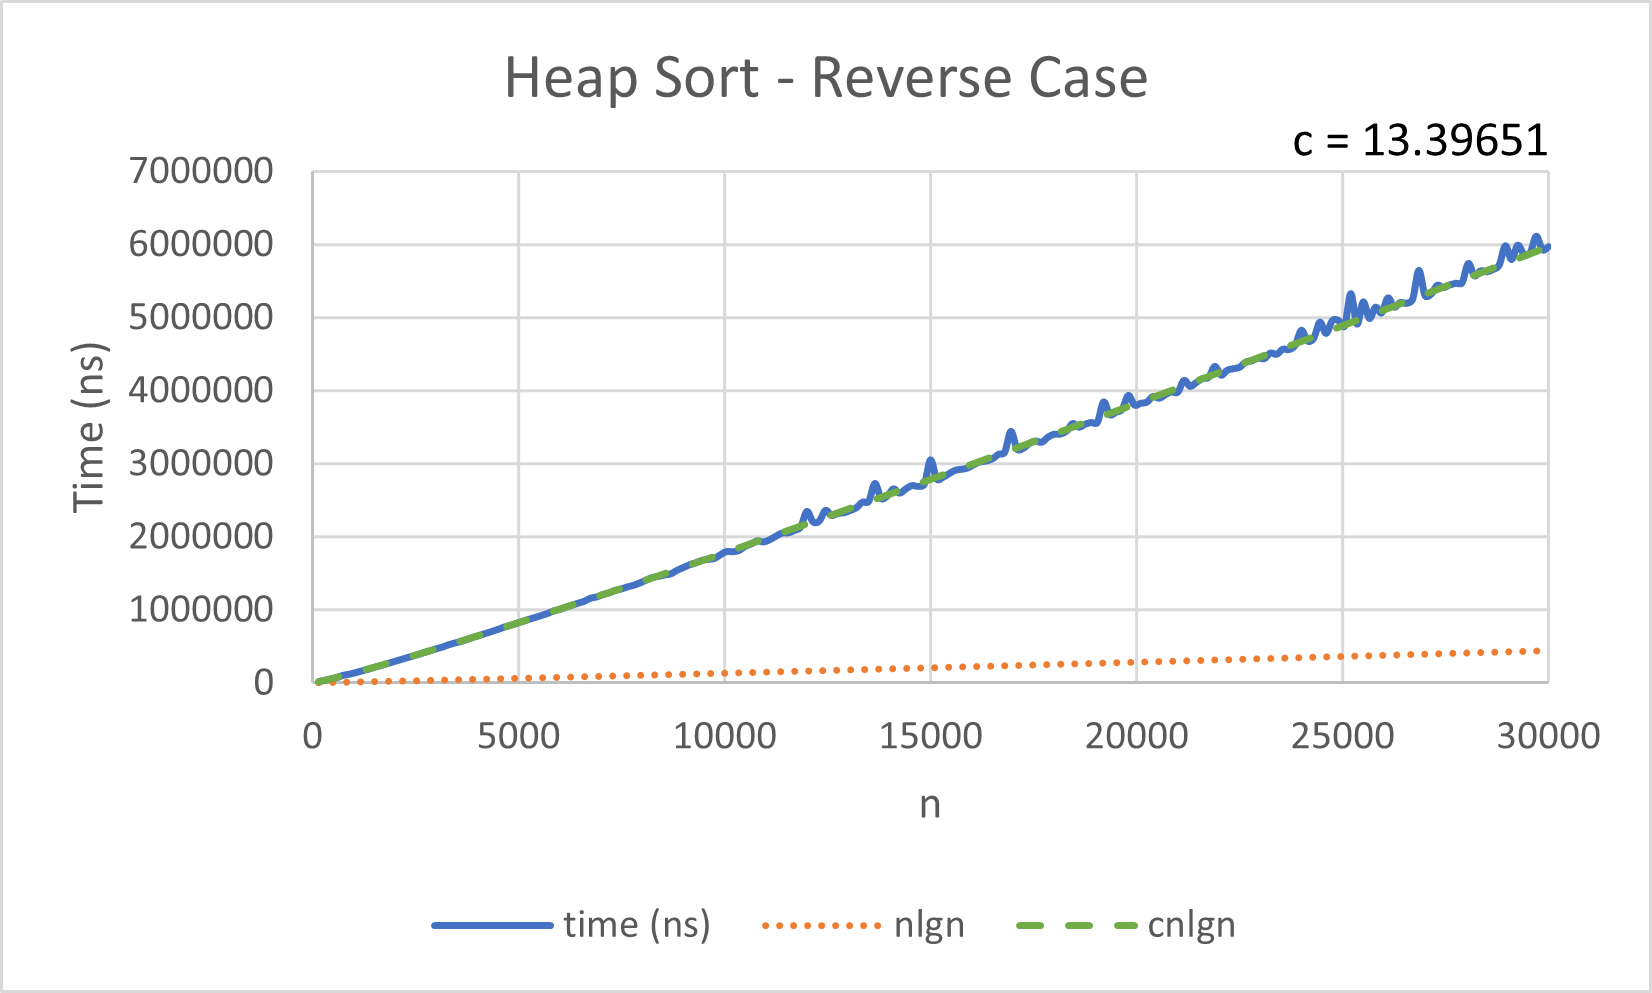
\includegraphics[width=0.9\linewidth]{heap_reverse.png}
				\caption{Heap Sort - Reverse Case}
				\label{graph:heap-reverse}
			\end{figure}
	\subsection{Quicksort}
		\paragraph{}
		The quicksort algorithm works by calling partitioning the array recursively by choosing the last element as the pivot. The sub-arrays are partitioned into three sections: values that are less than the pivot, values that are greater than the pivot, and the pivot. If the array is sorted or reversely sorted, the algorithm is substantially slower since the algorithm must go through every value of each sub-array since the largest or smallest is the pivot. One way to vastly increase the perform of quicksort is to implement a random pivot quicksort.
		\subsubsection{Random Case}
			\paragraph{}
			The results of quicksort sorting a random array is shown in Figure~\ref{graph:quick-random}. Quicksort on a random array is $O(cnlgn)$. As seen in Figure~\ref{graph:quick-random}, the constant value, $c$, is 10.37307. This value was found solving the equation $y=cnlgn$ where $y$ is the max time value and $n$ is max input value. In this case, $y=4628260$ and $n=30000$. The time function strays a little from the $cnlgn$ line; it is believe that this was caused from accessing the computer during this test while gathering data.
			\begin{figure}[H]
				\centering
				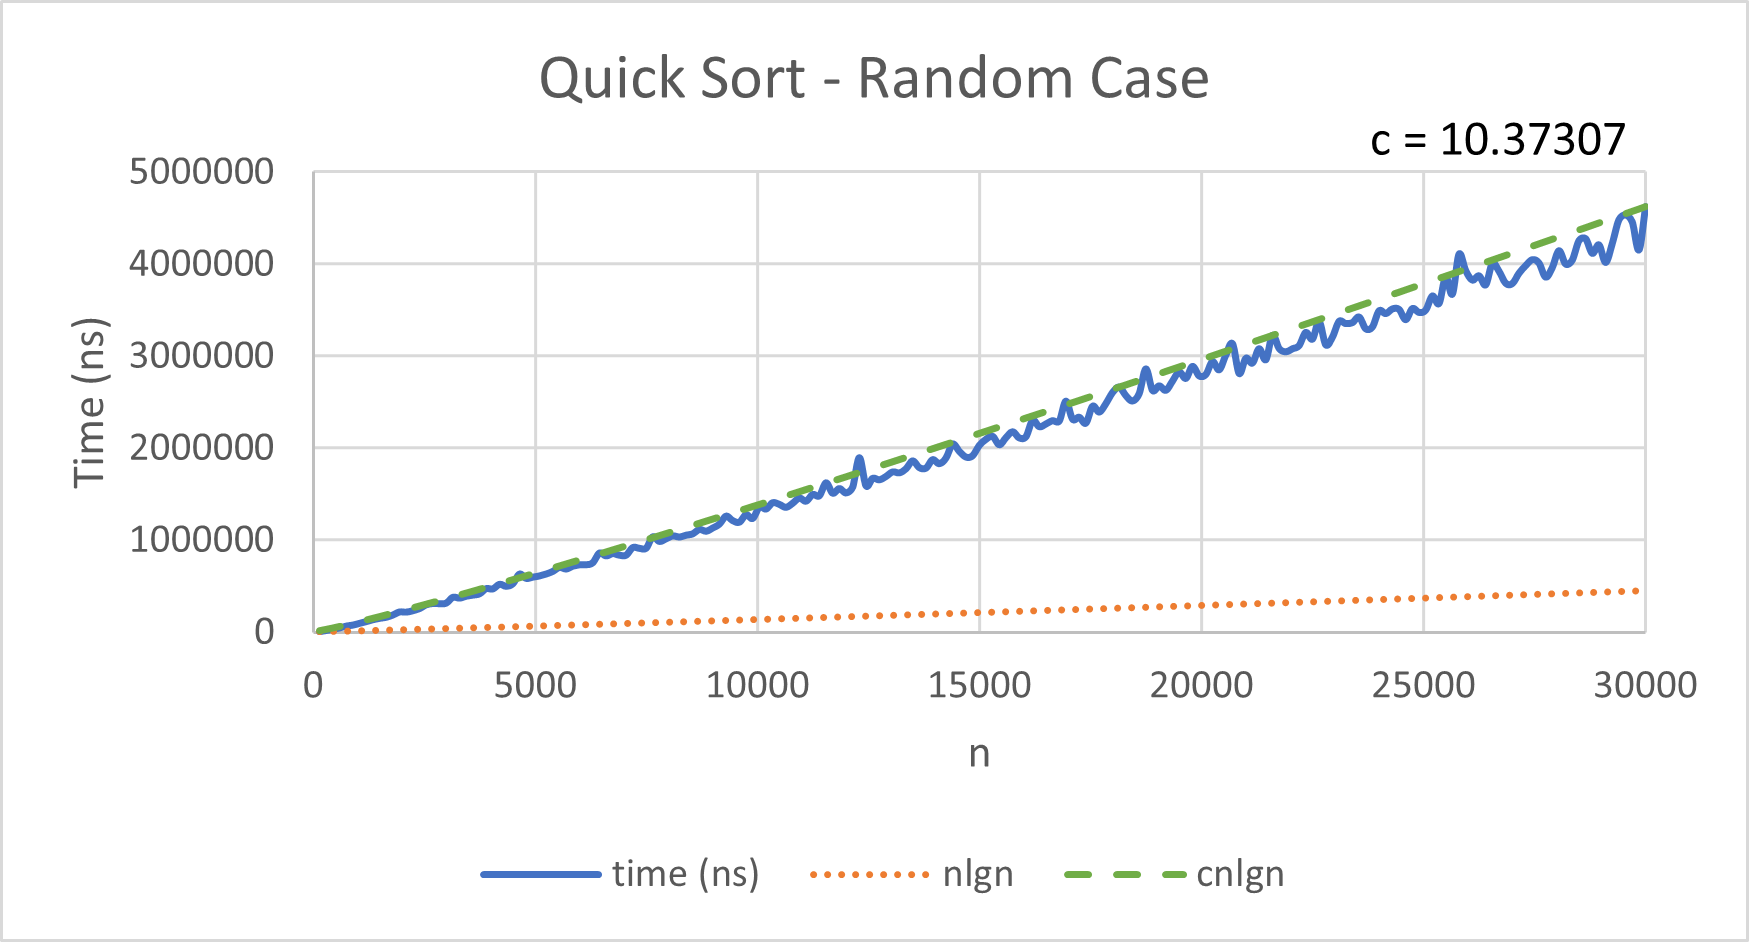
\includegraphics[width=0.9\linewidth]{quick_random.png}
				\caption{Quicksort - Random Case}
				\label{graph:quick-random}
			\end{figure}
		\subsubsection{Sorted Case}
			\paragraph{}
			The results of quicksort sorting a sorted array is shown in Figure~\ref{graph:quick-sorted}. Quicksort on a sorted array is $O(cn^2)$. As seen in Figure~\ref{graph:quick-sorted}, the constant value, $c$, is 2.965922. This value was found solving the equation $y=cn^2$ where $y$ is the max time value and $n$ is max input value. In this case, $y=2669330000$ and $n=30000$. Since $O(n^2)$ grows much faster than $O(nlgn)$, the constant from this case does not really matter since one of the other algorithms will perform better with a sorted data set. 
			\begin{figure}[H]
				\centering
				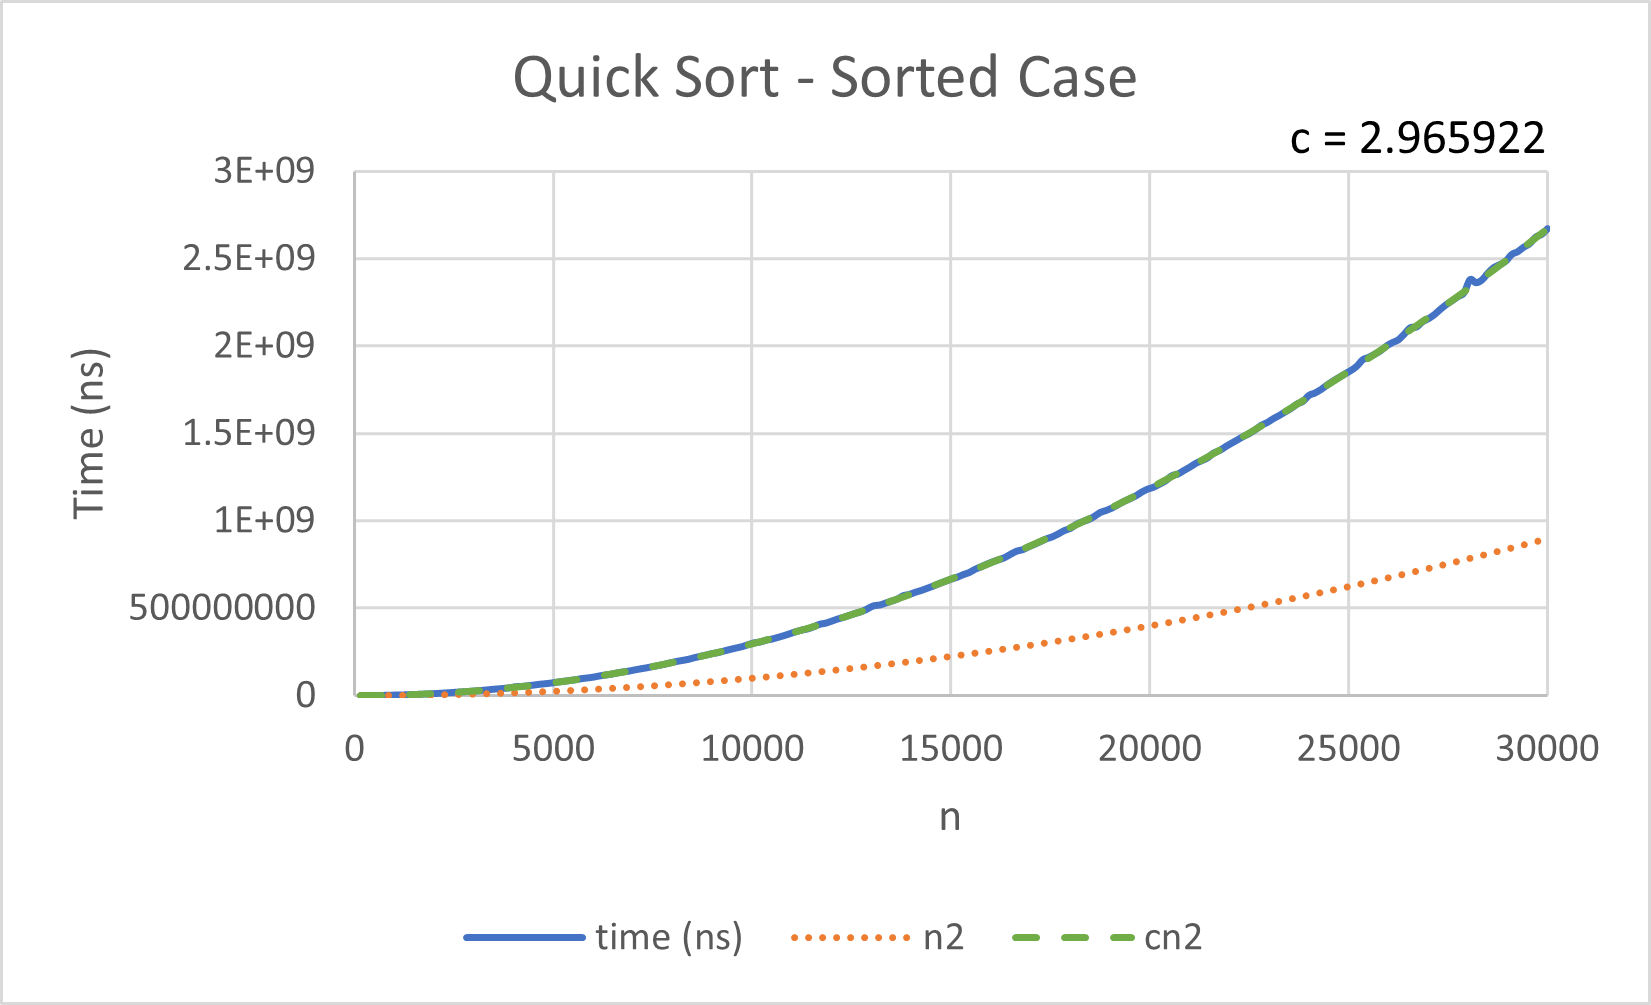
\includegraphics[width=0.9\linewidth]{quick_sorted.png}
				\caption{Quicksort - Sorted Case}
				\label{graph:quick-sorted}
			\end{figure}
		\subsubsection{Reverse Case}
			\paragraph{}
			The results of quicksort sorting a reversely-sorted array is shown in Figure~\ref{graph:quick-reverse}. Quicksort on a reversely-sorted array is $O(cn^2)$. As seen in Figure~\ref{graph:quick-reverse}, the constant value, $c$, is 2.048033. This value was found solving the equation $y=cn^2$ where $y$ is the max time value and $n$ is max input value. In this case, $y=1843230000$ and $n=30000$. Since $O(n^2)$ grows much faster than $O(nlgn)$, the constant from this case does not really matter since one of the other algorithms will perform better with a reversely-sorted data set.
			\begin{figure}[H]
				\centering
				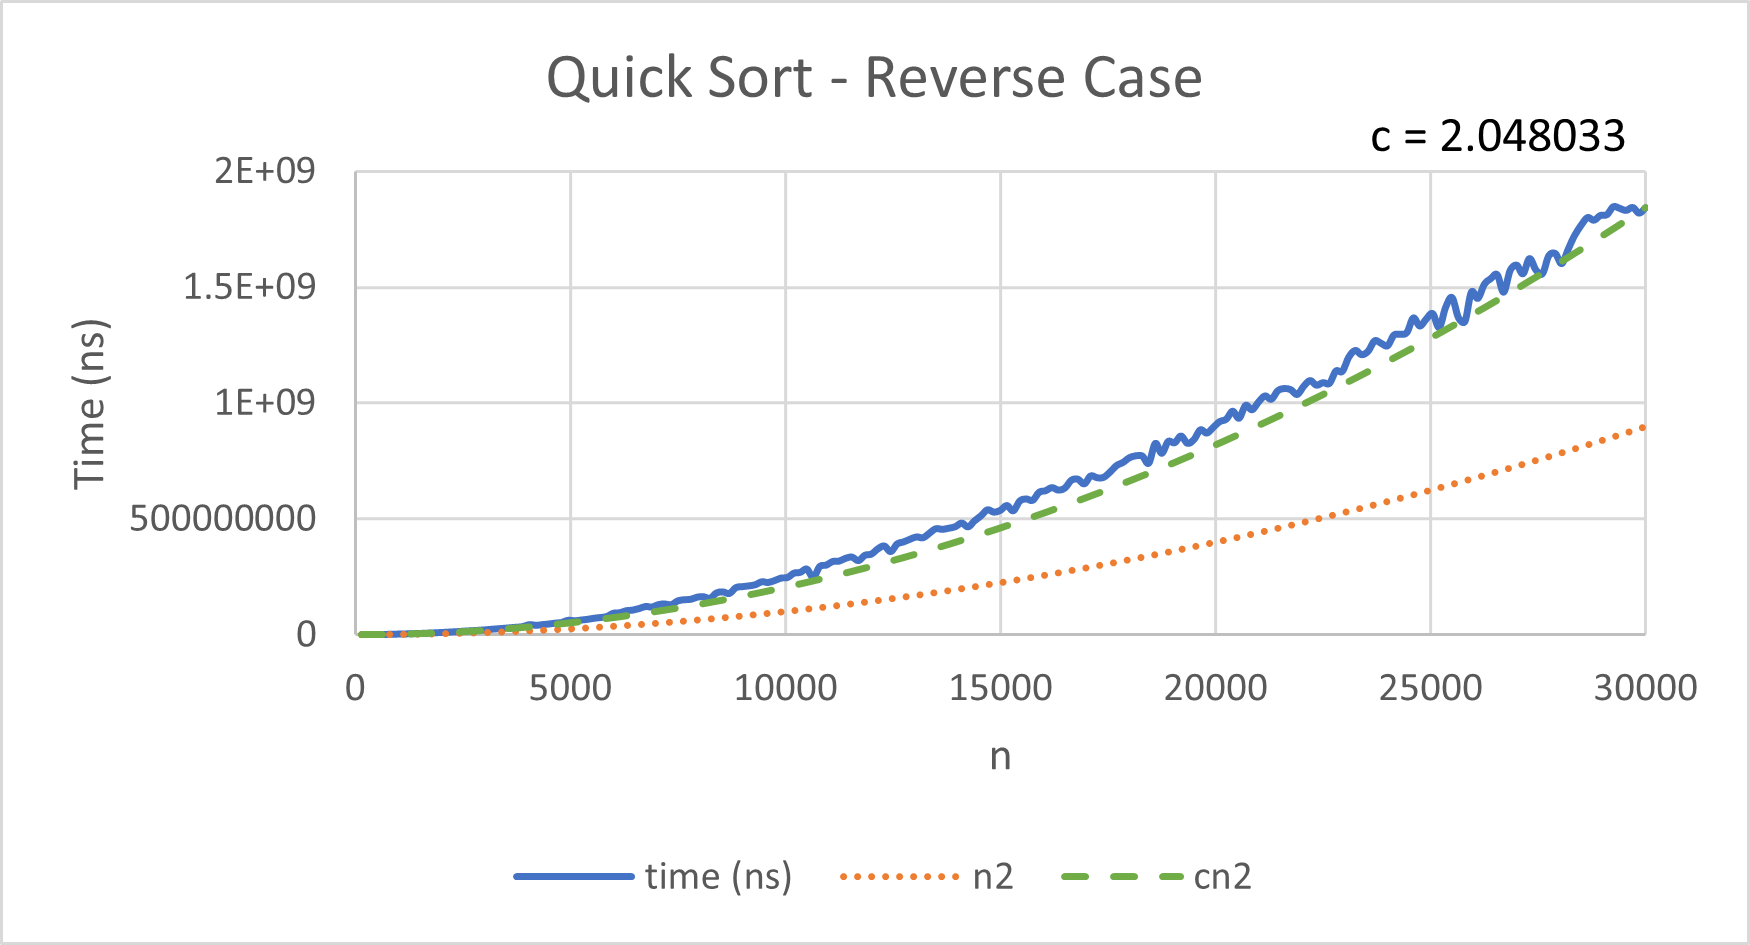
\includegraphics[width=0.9\linewidth]{quick_reverse.png}
				\caption{Quicksort - Reverse Case}
				\label{graph:quick-reverse}
			\end{figure}
	\subsection{Modified Merge Sort}
		\paragraph{}
		The modified merge sort implemented is merge insertion sort. The idea behind merge insertion sort is to find a input size, $n$, that makes insertion sort faster than merge sort. Once the sub-array are smaller than that input size, the algorithm will sort the sub-array with insertion sort and merge. In this report, input size 43 was the value found when insertion sort performed faster than merge sort.
		
		This subtly increased merge sorts performance if you compare the constants from each case. Merge sort's constants were 18.5962, 14.18871, and 14.102 from Figure~\ref{graph:merge-random}, Figure~\ref{graph:merge-sorted}, and Figure~\ref{graph:merge-reverse} respectfully. Meanwhile merge insertion sort's constants were 18.1225, 13.80608, and 14.09744 from Figure~\ref{graph:insertion-random}, Figure~\ref{graph:insertion-sorted}, and Figure~\ref{graph:insertion-reverse} respectfully.
		\subsubsection{Random Case}
			\paragraph{}
			The results of merge insertion sort sorting a random array is shown in Figure~\ref{graph:insertion-random}. Merge insertion sort on a random array is $O(cnlgn)$. As seen in Figure~\ref{graph:insertion-random}, the constant value, $c$, is 18.1225. This value was found solving the equation $y=cnlgn$ where $y$ is the max time value and $n$ is max input value. In this case, $y=8085900$ and $n=30000$. 
			\begin{figure}[H]
				\centering
				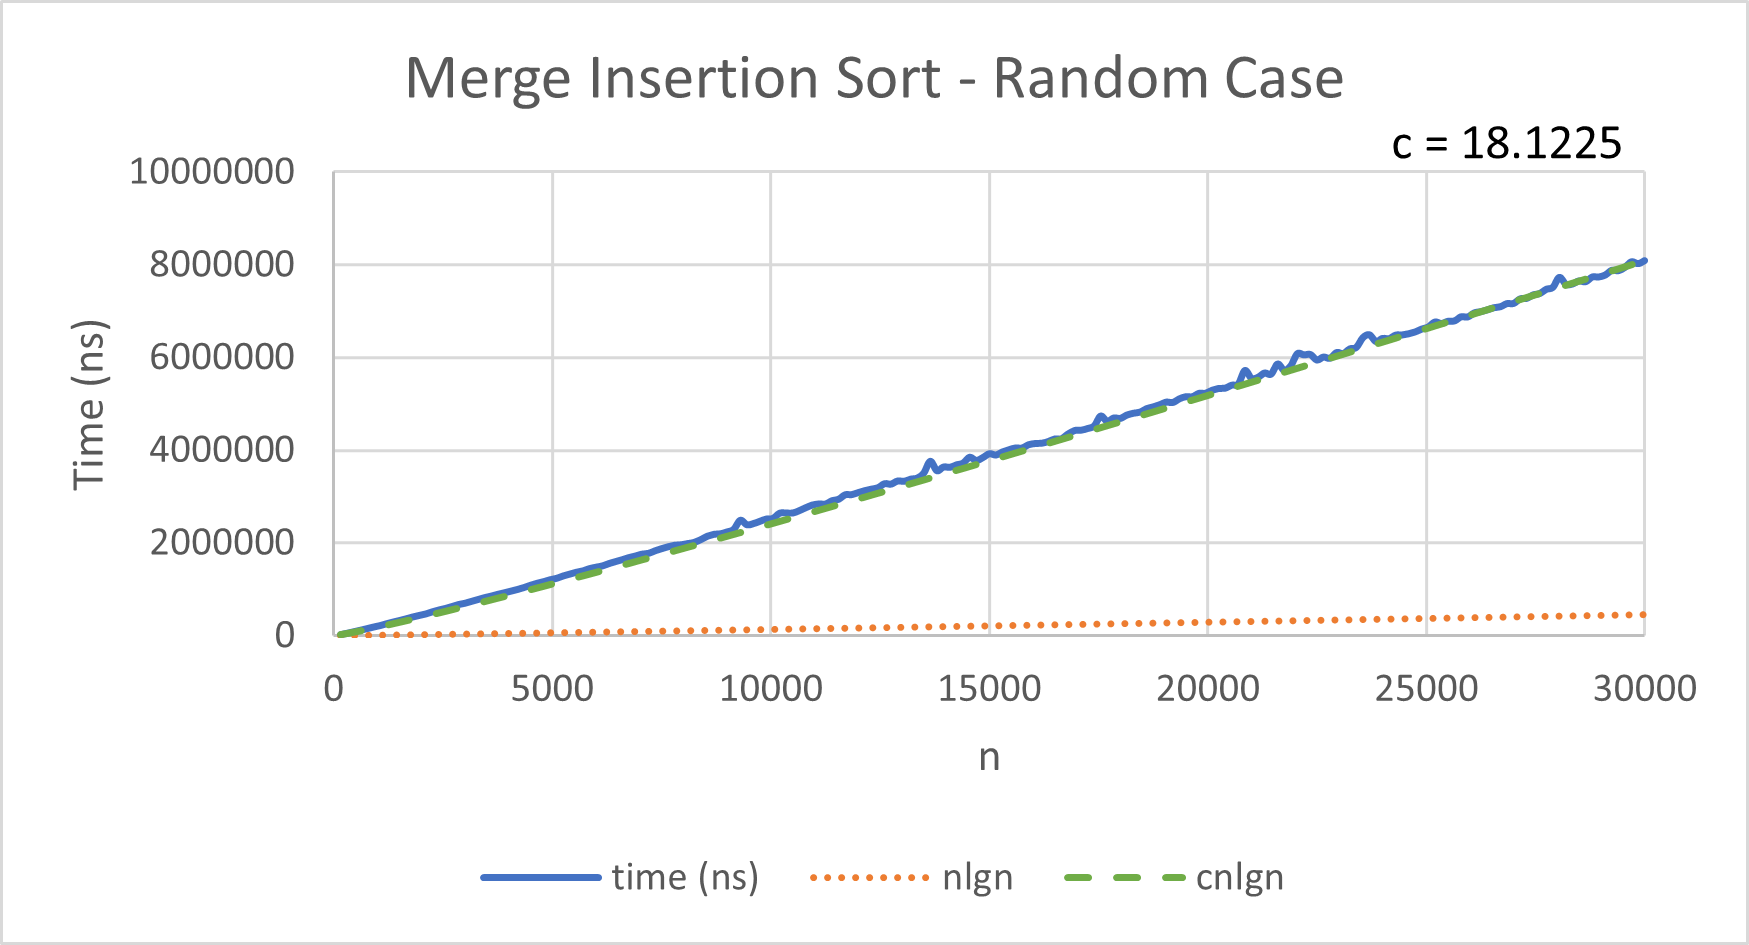
\includegraphics[width=0.9\linewidth]{insert_random.png}
				\caption{Merge Insertion Sort - Random Case}
				\label{graph:insertion-random}
			\end{figure}
		\subsubsection{Sorted Case}
			\paragraph{}
			The results of merge insertion sort sorting a sorted array is shown in Figure~\ref{graph:insertion-sorted}. Merge insertion sort on a sorted array is $O(cnlgn)$. As seen in Figure~\ref{graph:insertion-sorted}, the constant value, $c$, is 13.80608. This value was found solving the equation $y=cnlgn$ where $y$ is the max time value and $n$ is max input value. In this case, $y=6155170$ and $n=30000$. 
			\begin{figure}[H]
				\centering
				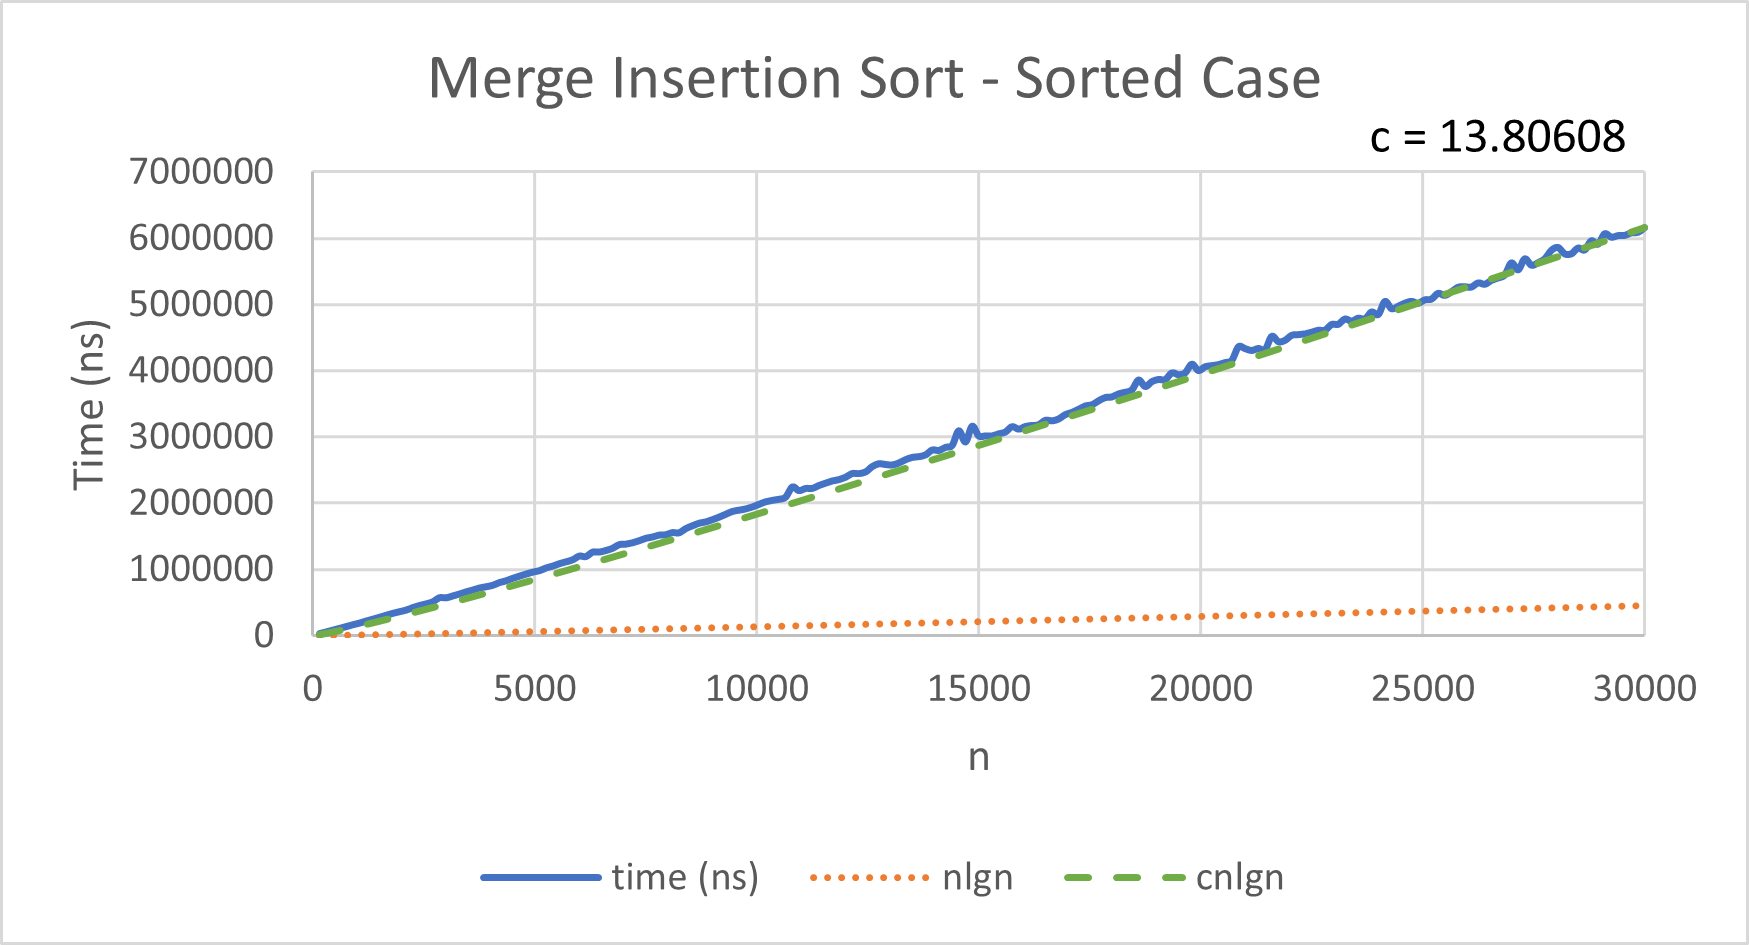
\includegraphics[width=0.9\linewidth]{insert_sorted.png}
				\caption{Merge Insertion Sort - Sorted Case}
				\label{graph:insertion-sorted}
			\end{figure}
		\subsubsection{Reverse Case} 
			\paragraph{}
			The results of merge insertion sort sorting a reversely-sorted array is shown in Figure~\ref{graph:insertion-reverse}. Merge insertion sort on a reversely-sorted array is $O(cnlgn)$. As seen in Figure~\ref{graph:insertion-reverse}, the constant value, $c$, is 14.09744. This value was found solving the equation $y=cnlgn$ where $y$ is the max time value and $n$ is max input value. In this case, $y=6290000$ and $n=30000$. 
			\begin{figure}[H]
				\centering
				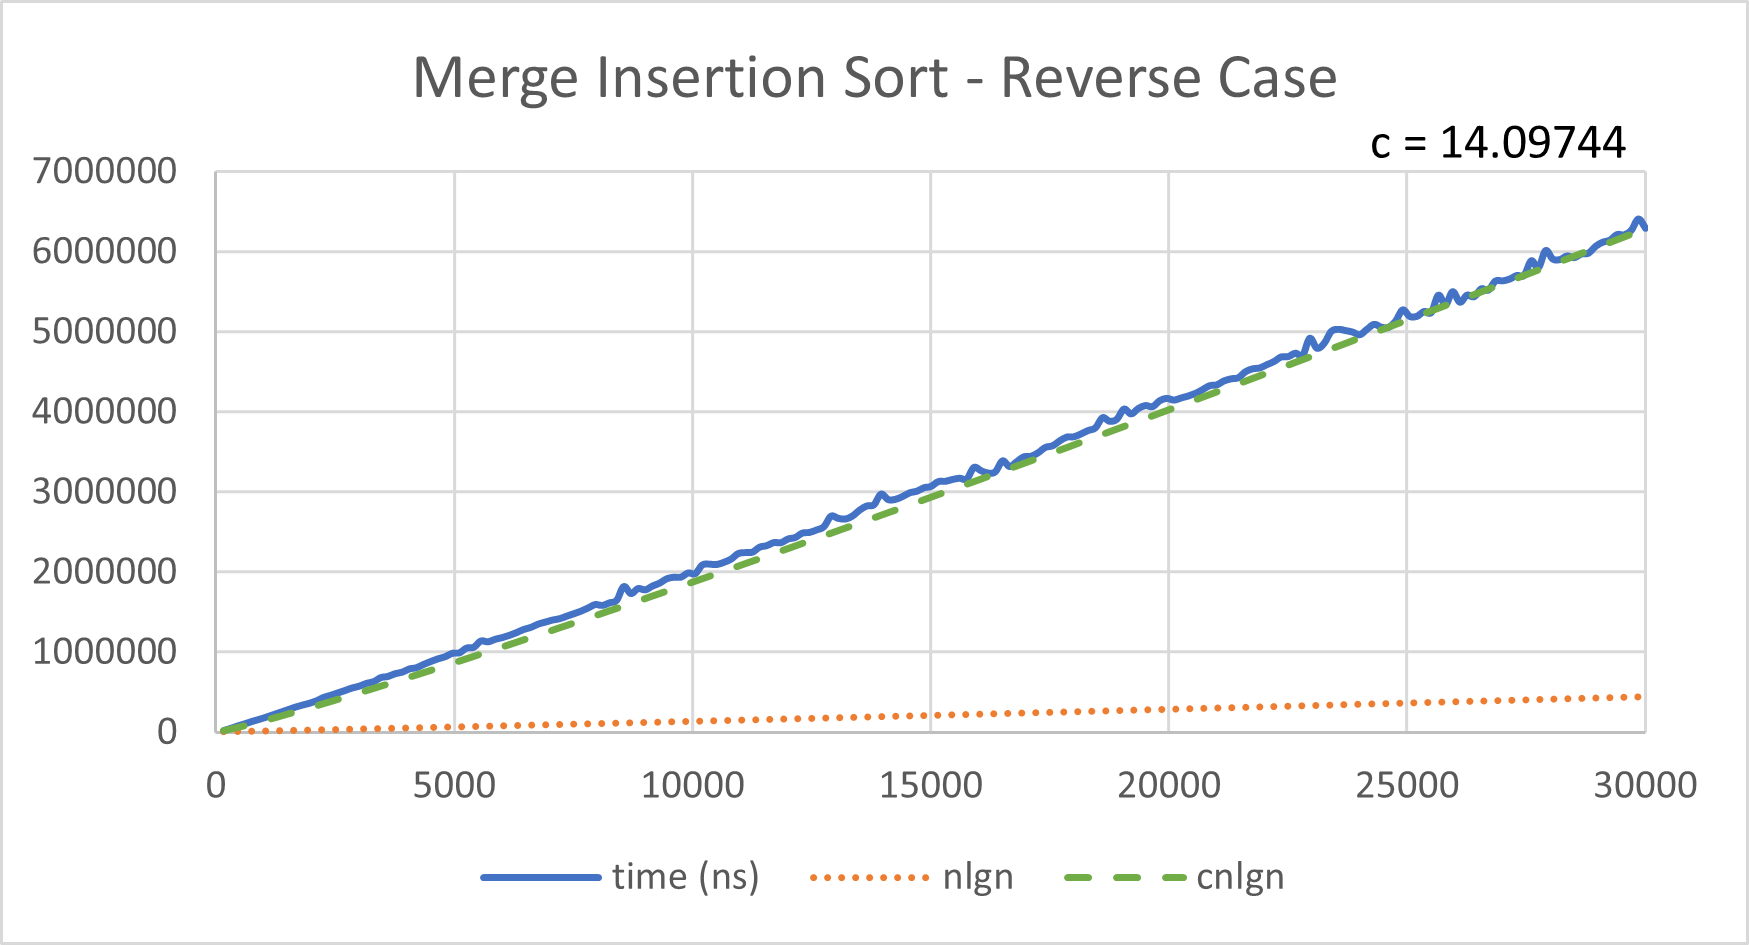
\includegraphics[width=0.9\linewidth]{insert_reverse.png}
				\caption{Merge Insertion Sort - Reverse Case}
				\label{graph:insertion-reverse}
			\end{figure}
\section{Conclusions}
	\paragraph{}
	Time complexity, among other quantities, of algorithms is important; it gives programmers an idea of how fast, or slow, an algorithm will take when input size becomes large. This report documented four algorithms' time complexity as input size grew large. Before analysis of results, the report showcased the algorithms' psuedocode to demonstrate how the algorithms work, how they are correct, and what pre and postconditions are expected. 
	
	Merge, heap, quick, and merge insertion sort were timed sorting a random, sorted, and reversely-sorted data set. For a random set of data, quick sort performed the best with a leading constant of 10.37307 (Figure~\ref{graph:quick-random}). For a sorted set of data, merge insertion sort performed the best with a leading constant of 13.80608 (Figure~\ref{graph:insertion-sorted}). For a reversely-sorted set of data, heap sort performed the best with a leading constant of 13.39651 (Figure~\ref{graph:heap-reverse}). The guess at the beginning of the report was almost correct. Instead of merge sort being best for reversely-sorted data, it was heap sort.
	
	If only one sort were to be picked, quick sort is the best sort out of the tested sorts. While its performance with sorted and reversely-sorted data sets was abysmal, implementing a quick sort where the pivot is randomly chosen instead of being the last element in the sub-array will change its performance similar of that of a random data set, which was the best performing out of all of the sorts.
	

\begin{thebibliography}{9}
	\bibitem{cormen2001introduction}
	T.~H. Cormen, C.~E. Leiserson, R.~L. Rivest, C.~Stein.,
	\emph{{Introduction to Algorithms, 3rd Edition}}.
	MIT press Cambridge, 2001.
\end{thebibliography}
\newpage
\section*{Appendix A}
	\large{\textbf{CPP Source Code: main.cpp}}
	\tiny{\lstinputlisting{main.cpp}}
	\large{\textbf{CPP Source Code: algorithmManager.h}}
	\tiny{\lstinputlisting{algorithmManager.h}}
	\large{\textbf{CPP Source Code: algorithmManager.hpp}}
	\tiny{\lstinputlisting{algorithmManager.hpp}}
\end{document}